% $Header: /cvsroot/latex-beamer/latex-beamer/solutions/generic-talks/generic-ornate-15min-45min.en.tex,v 1.5 2007/01/28 20:48:23 tantau Exp $

\documentclass{beamer}

\usepackage{caption}
\captionsetup{labelformat=empty,labelsep=none,font=scriptsize}
\setlength{\abovecaptionskip}{0pt}

\usepackage{color}
%% These definitions are based on darkred at
%% http://www.december.com/html/spec/colorcmyk.html
\definecolor{darkred}{cmyk}{0, 1, 1, 0.45}
\newcommand{\jul}{\textcolor{darkred}}
\newcommand{\jan}{\textcolor{blue}}

% This file is a solution template for:

% - Giving a talk on some subject.
% - The talk is between 15min and 45min long.
% - Style is ornate.



% Copyright 2004 by Till Tantau <tantau@users.sourceforge.net>.
%
% In principle, this file can be redistributed and/or modified under
% the terms of the GNU Public License, version 2.
%
% However, this file is supposed to be a template to be modified
% for your own needs. For this reason, if you use this file as a
% template and not specifically distribute it as part of a another
% package/program, I grant the extra permission to freely copy and
% modify this file as you see fit and even to delete this copyright
% notice. 


\mode<presentation>
{
  \usetheme{Warsaw}
  % or ...

  \setbeamercovered{transparent}
  % or whatever (possibly just delete it)
}


\usepackage[english]{babel}
% or whatever

\usepackage[latin1]{inputenc}
% or whatever

\usepackage{times}
\usepackage[T1]{fontenc}
% Or whatever. Note that the encoding and the font should match. If T1
% does not look nice, try deleting the line with the fontenc.


%% \title[Short Paper Title] % (optional, use only with long paper titles)
%% {Presentation Title}
%% \title[]{Initial findings}
%\subtitle {Eastern CASTNET sites, May-Sep.~2001} % (optional)

%% \author[Author, Another] % (optional, use only with lots of authors)
%% {F.~Author\inst{1} \and S.~Another\inst{2}}
%% % - Use the \inst{?} command only if the authors have different
%% %   affiliation.
%% \author[Swall et al.]{Jenise Swall\inst{1}, Ana Rappold\inst{2}, and Lucas Neas\inst{2}
% - Use the \inst{?} command only if the authors have different
%   affiliation.

%% \institute[Universities of Somewhere and Elsewhere] % (optional, but mostly needed)
%% {
%%   \inst{1}%
%%   Department of Computer Science\\
%%   University of Somewhere
%%   \and
%%   \inst{2}%
%%   Department of Theoretical Philosophy\\
%%   University of Elsewhere}
%% % - Use the \inst command only if there are several affiliations.
%% % - Keep it simple, no one is interested in your street address.
 %% \institute[VCU]
 %% {
 %%   \inst{1}%
 %%   Dept.\ of Statistical Sciences and Operations Research\\
 %%   Virginia Commonwealth University
 %%   \and
 %%   \inst{2}%
 %%   National Health and Environmental Effects Research Laboratory\\
 %%   U.S.~Environmental Protection Agency
 %% }

%% \date[Short Occasion] % (optional)
%% {Date / Occasion}
\date{May 2021}

%% \subject{Talks}
% This is only inserted into the PDF information catalog. Can be left
% out. 



% If you have a file called "university-logo-filename.xxx", where xxx
% is a graphic format that can be processed by latex or pdflatex,
% resp., then you can add a logo as follows:

% \pgfdeclareimage[height=0.5cm]{university-logo}{university-logo-filename}
% \logo{\pgfuseimage{university-logo}}



% Delete this, if you do not want the table of contents to pop up at
% the beginning of each subsection:
\AtBeginSection[]
{
  \begin{frame}<beamer>{Outline}
    \tableofcontents[currentsection,currentsubsection]
  \end{frame}
}


% If you wish to uncover everything in a step-wise fashion, uncomment
% the following command: 

%\beamerdefaultoverlayspecification{<+->}

\useoutertheme{infolines}

\begin{document}

%% \begin{frame}
%%   \titlepage
%% \end{frame}

\begin{frame}{Outline}
  \tableofcontents
  % You might wish to add the option [pausesections]
\end{frame}


% Since this a solution template for a generic talk, very little can
% be said about how it should be structured. However, the talk length
% of between 15min and 45min and the theme suggest that you stick to
% the following rules:  

% - Exactly two or three sections (other than the summary).
% - At *most* three subsections per section.
% - Talk about 30s to 2min per frame. So there should be between about
%   15 and 30 frames, all told.


%% %%%%%%%%%%%%%%%%%%%%%%%%%%%%%%%%%%%%%%%%%%%%%%%%%%%%%%%%%%



%% %%%%%%%%%%%%%%%%%%%%%%%%%%%%%
%% Introductory material
%% \section[Background]{Background ideas and info}
\section[Preparation]{Preparing the data}



\begin{frame}{Percentages unclassified at the family level}

  \begin{center}
    \begin{figure}
      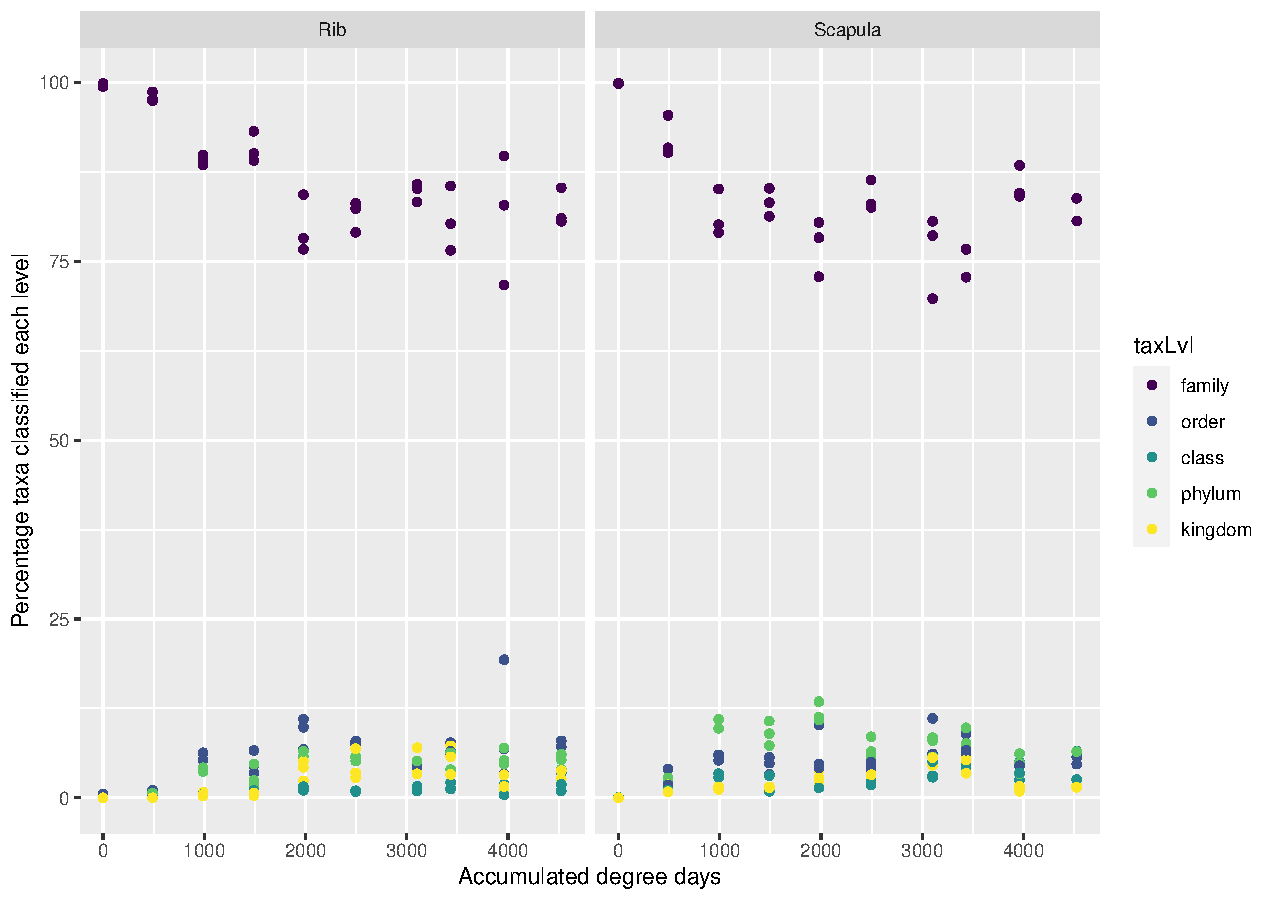
\includegraphics[width=3.25in]{swabs_family_perc_classif_by_add_type}
    \end{figure}
  \end{center}
  \vspace{-0.1in}
  {\footnotesize
  Fractions classified to family level:
  \begin{itemize}
    \item Ribs: 86.8\% (vs.\ 90.5\% for bones)
    \item Scapulae: 83.2\% (vs.\ 88.9\% for bones)
  \end{itemize}
  }
\end{frame}


\begin{frame}{Which taxa were included?}

  \begin{itemize}
  \item For each sample, we calculated the total counts of all classified,
family-level taxa.
  \item For each sample, we calculated the fraction of counts
associated with each family-level taxa. 
  \item To be included in the family-level analysis, we require that a taxon
  makes up more than 1\% of the total counts for at least 2 samples.
  \end{itemize}

  \vspace{0.1in}

  \noindent This is similar to the process we used when setting up for the
analyses in the Forger et al.~ paper, but I'm open to revisiting it.

  \vspace{0.1in}

  \noindent Number of taxa utilized in random forest models:
  \begin{itemize}
    \item Ribs: 21 taxa (vs.\ 24 used for earlier bone analysis)
    \item Scapulae: 37 taxa (vs.\ 34 used for earlier bone analysis)
  \end{itemize}


\end{frame}
%% %%%%%%%%%%%%%%%%%%%%%%%%%%%%%



%% %%%%%%%%%%%%%%%%%%%%%%%%%%%%%
\section[Rib swabs]{Working with swabs from ribs}


\begin{frame}{Implementing the random forest model for ribs}

Full model using baseline observations (ADD 0):
\begin{itemize}
  \item Utilized 21 family-level taxa.
  \item RMSE: 577.5 $\pm$  11.4
  \item Explained variation: 83.9\%
$\pm$ 0.6\%
  \item Not as precise as the analysis for rib bones - maybe due to fewer
observations.
\end{itemize}

\vspace{0.1in}

If we run the model without the baseline observations, we have:\\
\noindent RMSE: 609.2 $\pm$ 11.1 \hspace{0.05in}  Explained variation: 77.9\%
$\pm$ 0.8\%\\
\vspace{0.05in}
The following graphs are from the model using baseline observations.

\end{frame}



\begin{frame}{Which taxa are influential in the random forest model?}

  \begin{center}
    \begin{figure}
      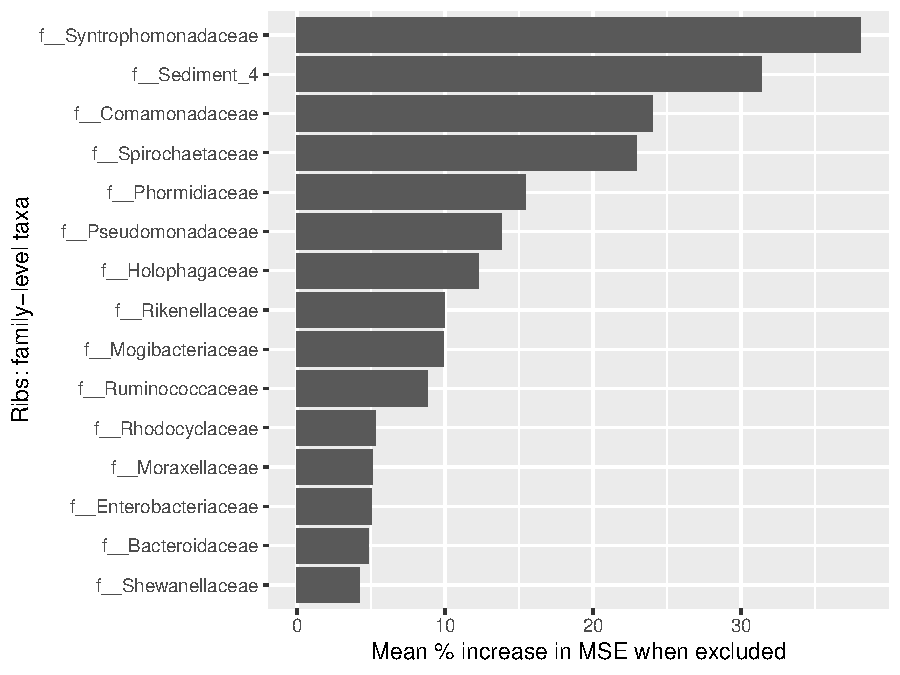
\includegraphics[width=3.25in]{use_families/w_ribs/w_baseline/families_rib_PercIncMSE_barchart}
    \end{figure}
  \end{center}
  \vspace{-0.1in}
  \scriptsize{
  \begin{itemize}
    \item The measure of importance is the mean percentage increase in the
    mean-square error of model predictions when the variable is left out of the
    model. 
    \item I've shown the top 15 because they'd fit, but 21 were used in the
    model.
  \end{itemize}
  }

\end{frame}



\begin{frame}{Scatterplots for influential taxa}

  \begin{center}
    \begin{figure}
      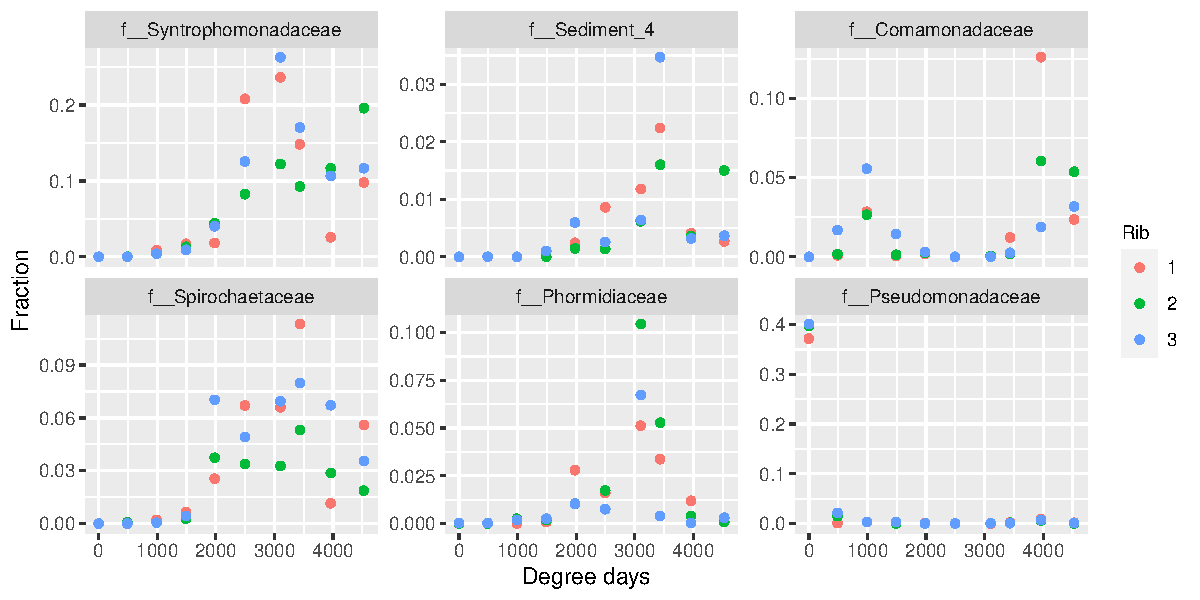
\includegraphics[width=4.75in]
        {use_families/w_ribs/w_baseline/infl_rib_family_scatter}
    \end{figure}
  \end{center}
  \vspace{-0.25in}
  \scriptsize{
  \begin{itemize}
    \item I've only shown top 6 due to spacing constraints.
    \item Note that the y-axes have differing scales.
    \item Fractions of Sediment\_4, Comamonadaceae, and Spirochaetaceae are very
    low.
  \end{itemize}
  }

\end{frame}



\begin{frame}{Getting a sense of "real-life" model fit}

  \noindent In real life, we would be estimating ADD without
  \begin{itemize}
    \item having seen that rib/scapula before, and
    \item maybe not having observed any rib/scapula at that level of ADD before
  \end{itemize} 

  \vspace{0.1in}

  \noindent To try to get a sense of how the model would work in such cases, I
  \begin{itemize}
    \item fitted the model over and over, each time without one particular
    combination of rib/scapula number and ADD.
    \item This means the model had no info about the left-out rib/scapula and no
    info about bacteria counts at that ADD.
    \item Then, I used the model to estimate the ADD for the left-out
    rib/scapula for the left-out ADD.
  \end{itemize}
  
\end{frame}



\begin{frame}{Residual plot to get sense of "real-life" model fit}

  \begin{center}
    \begin{figure}
      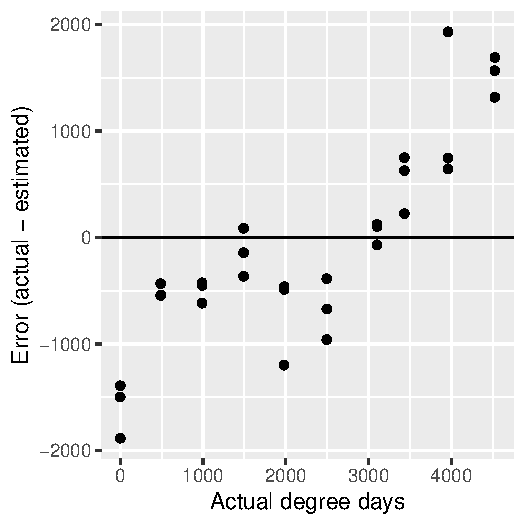
\includegraphics[width=2.2in]
        {use_families/w_ribs/w_baseline/leave_out_one_rib_and_one_day_residuals}
      \caption{Residuals when leaving out one rib and one ADD at a time}
    \end{figure}
  \end{center}
  \vspace{-0.1in}
\scriptsize{
\begin{itemize}
  \item This RMSE is about 926, which is higher than the RMSE for the full
  dataset (as expected).  We have less data available for each run, and we're
  predicting for an ADD value which we have no information about.
  \item The errors tend to be larger at the extremes.
\end{itemize}
}

\end{frame}
% %%%%%%%%%%%%%%%%%%%%%%%%%%%%%




% %%%%%%%%%%%%%%%%%%%%%%%%%%%%%
\section[Scapula swabs]{Working with swabs from scapulae}

\begin{frame}{Implementing the random forest model for scapulae}

\begin{itemize}
  \item The model utilized 37 family-level taxa.
  \item RMSE: 589.5 $\pm$ 18.3
  \item Explained variation: 81.2\% $\pm$ 1.2\%
\end{itemize}

\vspace{0.1in}

If we run the model without the baseline observations, we have:\\
\noindent RMSE: 522.0 $\pm$ 13.0 \hspace{0.05in}  Explained variation: 82.7\%
$\pm$ 0.9\%\\
\vspace{0.05in}
The following graphs are from the model using baseline observations.

\end{frame}


\end{document}


\begin{frame}{Which taxa are influential in the random forest model?}

  \begin{center}
    \begin{figure}
      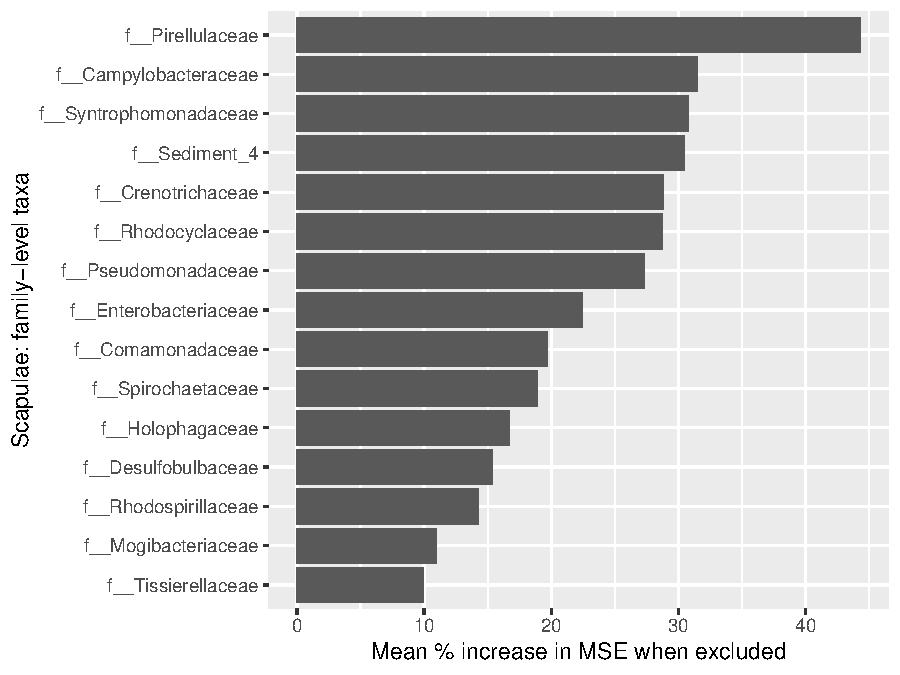
\includegraphics[width=3.25in]{use_families/w_scapulae/families_scapula_PercIncMSE_barchart}
    \end{figure}
  \end{center}
  \vspace{-0.1in}
  \scriptsize{
  \begin{itemize}
  \item I've shown 15 because they would fit, but 34 were used in the model.
  \item The first 7-8 taxa are noticeably more influential than those that
  follow.
  \end{itemize}
  }

\end{frame}



\begin{frame}{Scatterplots for influential taxa}

  \begin{center}
    \begin{figure}
      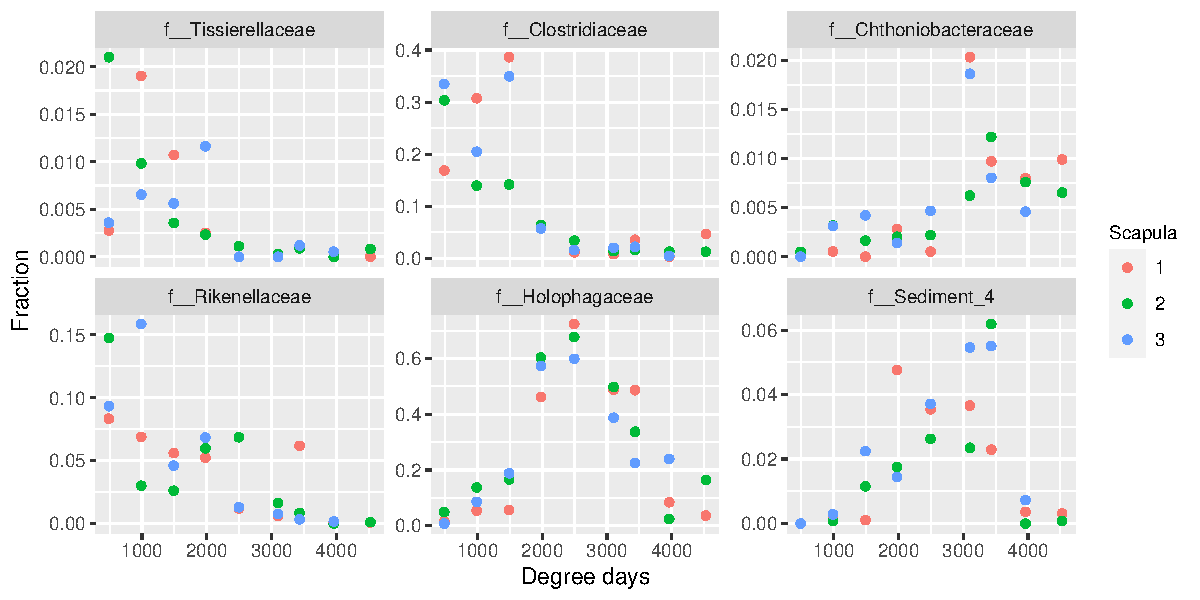
\includegraphics[width=4.75in]{use_families/w_scapulae/infl_scapula_family_scatter}
    \end{figure}
  \end{center}
  \vspace{-0.25in}
  \scriptsize{
  \begin{itemize}
  \item I've only shown top 6 because more than that is hard to fit.
  \item Note that the y-axes have differing scales.
  \item Fractions of Pirellulaceae, Campylobacteraceae, and Crenotrichacea
  are very low.
  \end{itemize}
  }

\end{frame}



\begin{frame}{Residual plot to get sense of "real-life" model fit}

  \begin{center}
    \begin{figure}
      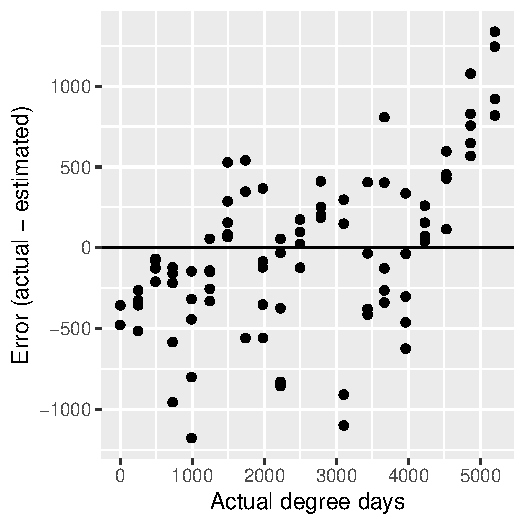
\includegraphics[width=2.2in]{use_families/w_scapulae/leave_out_one_scapula_and_one_day_residuals}
      \caption{Residuals when leaving out one scapula and one ADD at a time}
    \end{figure}
  \end{center}
  \vspace{-0.1in}
\scriptsize{
\begin{itemize}
  \item This RMSE is 452.7, which is higher than the RMSE for the full
  dataset (as you'd expect).  We have less data available for each run, and we're predicting for an
  ADD value which we have no information about.
  \item The errors tend to be larger at the extremes.
\end{itemize}
}
\end{frame}
%% %%%%%%%%%%%%%%%%%%%%%%%%%%%%%

\end{document}
